\chapter{Parte 1}\label{parte_1}

O pacote de $scripts$ para o modelo de $Lattice$ $Boltzmann$ proposto se divide nos seguintes arquivos:
\begin{itemize}
	\item main\_lbgk.m: $script$ responsável pelo fluxo principal e pela leitura e alocação de constantes físicas macroscópicas e mesoscópicas da $lattice$.
	\item build\_lattice\_D2Q9.m: $script$ responsável por construir a estrutura de dados $struct$ para comportar as matrizes de densidades e suas respectivas velocidades;
	\item set\_initial\_disturbances.m: $script$ responsável por configurar uma perturbação inicial no sistema de $lattice$;
	\item stream\_lattice.m: $script$ responsável por descolar as células de $lattice$ e recalcular as velocidades;
	\item collide\_lattice.m: $script$ responsável por calcular as funções de relaxamento e colidir as células de densidade da $lattice$;
\end{itemize}

\section{$Script$ de fluxo principal: main\_lbgk.m}
Esse $script$ segue o seguinte fluxo:
\begin{enumerate}
	\item São setados as dimensões da $lattice$;
	\item São setados e calculados os parâmetros físicos de natureza macroscópica;
	\item São setados e calculados os parâmetros próprios da $lattice$ de natureza mesoscópica;
	\item A estrutura de dados $lattice$ é criada a partir da função build\_lattice\_D2Q9.m;
	\item Uma perturbação inicial é criada dentro da $lattice$ através da função \\ set\_initial\_disturbances.m;
	\item O processo iterativo principal começa e dentro dele há:
		\begin{enumerate}
			\item Propagação de células através da função stream\_lattice.m;
			\item Extração da densidade da $lattice$;
			\item Colisão das células de $lattice$ através da função collide\_lattice.m.
		\end{enumerate}
\end{enumerate}
\begin{lstlisting}
% 2D Lattice Boltzmann (BGK) model of a fluid.
%  c4  c3   c2  D2Q9 model. At each timestep, particle densities propagate
%    \  |  /    outwards in the directions indicated in the figure. An
%  c5 -c9 - c1  equivalent 'equilibrium' density is found, and the densities
%    /  |  \    relax towards that state, in a proportion governed by omega.
%  c6  c7   c8      Iain Haslam, March 2006.

clear all, clc
close all

%% 1 - Set lattice sizes
number_lines_lattice = 300; % cells in the y direction
number_columns_lattice = 300; % cells in the x direction

%% 2 - Set physical parameters (macro)
physical_sound_velocity = 340; % [m/s]
physical_density = 1.2; % [kg/m^3]
physical_dimension_max_x = .5; % [m]
physical_dimension_max_y = .5; % [m]
% voxel is a term to express a volume decribed in a pixel: volume + pixel = voxel
dimension_x_voxel = physical_dimension_max_x/number_columns_lattice; % defining dimension x in voxel
lattice_time_step = (1/sqrt(3))*dimension_x_voxel/physical_sound_velocity;

%% 3 - Set lattice parameters (meso - lattice unities)
frequency_relaxation = 1.9;
time_relaxation = 1/frequency_relaxation;
lattice_average_density = 1;
lattice_sound_speed = 1/sqrt(3);
lattice_sound_speed_pow_2 = lattice_sound_speed^2;
lattice_viscosity = lattice_sound_speed_pow_2*(1/frequency_relaxation-0.5);
physical_viscosity = lattice_viscosity*(dimension_x_voxel^2)/lattice_time_step; % [m^2/s]

% 4 - Build lattice struct with D2Q9
lattice = build_lattice_D2Q9(number_lines_lattice, number_columns_lattice, lattice_average_density);

% 5 - Set initial disturbance
initial_disturbance_density = 0.01;
lattice = set_initial_disturbances(lattice, initial_disturbance_density);

%% 6 - Begin the iteractive process
frequency_source = 1000; % Hz
amplitude_source = 0.001;
for ta = 1 : 150*sqrt(3)
    
    %% 6.1 - Propagation (streaming)
    lattice = stream_lattice(lattice);

    %% 6.2 - Get density
    lattice_distribution = lattice{1};
    density_total = sum(lattice_distribution,3);

    %% 6.3 - Collide
    lattice = collide_lattice(lattice, frequency_relaxation);
    
% Ploting the results in real time   
surf(density_total - 1), view(2), shading flat, axis equal, caxis([-.00001 .00001])
grid off
pause(.0001) 

end %  End main time Evolution Loop
\end{lstlisting}


\section{$Script$ de criação de lattice: build\_lattice\_D2Q9.m}
Esse $script$ segue o seguinte fluxo:
\begin{enumerate}
	\item É criado uma matriz de densidade da $lattice$ com valores 0 dado o número de linhas, colunas e direções de velocidade de propagação do modelo D2Q9;
	\item Essa matriz é preenchida com valores da densidade média do flúido;
	\item As velocidades em $x$ e em $y$ são criadas com valores de 0;
	\item A matriz de densidade e as velocidades são acopladas a estrutura de dados principal $lattice$ do tipo $struct$.
\end{enumerate}
\lstinputlisting{../code_matlab/code_refactored/build_lattice_D2Q9.m}

\section{$Script$ de criação de perturbações iniciais: \\ set\_initial\_disturbances.m}
O seguinte $script$ possui somente um bloco principal de código que faz com que uma perturbação de entrada na função seja colocada no centro geométrico do campo do flúido.
\lstinputlisting{../code_matlab/code_refactored/set_initial_disturbances.m}

\section{$Script$ de propagação das células de $lattice$: stream\_lattice.m}
Esse $script$ segue o seguinte fluxo:
\begin{enumerate}
	\item Informações de número máximo de linhas, colunas e matriz de distribuição de densidades são extraídas da estrutura de dados principal $lattice$;
	\item Os pontos de densidades são propagados nas direções postulados pelo modelo D2Q9;
	\item As velocidades são recalculadas de acordo com o modelo D2Q9;
	\item A matriz de densidade e as velocidades são acopladas a estrutura de dados principal $lattice$ do tipo $struct$.
\end{enumerate}
\lstinputlisting{../code_matlab/code_refactored/stream_lattice.m}

\section{$Script$ de colisão das células de $lattice$: collide\_lattice.m}
Esse $script$ segue o seguinte fluxo:
\begin{enumerate}
	\item Informações de número máximo de linhas, colunas, matriz de distribuição de densidades e velocidades são extraídas da estrutura de dados principal $lattice$;
	\item Constantes numéricas postuladas no modelo D2Q9 são setadas para a construção da matriz de relaxação;
	\item As funções de relaxação são calculadas de acordo com as velocidades e constantes do modelo D2Q9;
	\item Dada a matriz de distribuição de densidades, o cálculo de colisão é feito. Após matriz de distribuição de densidades é acoplada a estrutura de dados principal $lattice$ do tipo $struct$.
\end{enumerate}
\lstinputlisting{../code_matlab/code_refactored/collide_lattice.m}

%\begin{figure}[h!]
%    %\centering
%    \hspace{-4.5cm}
%    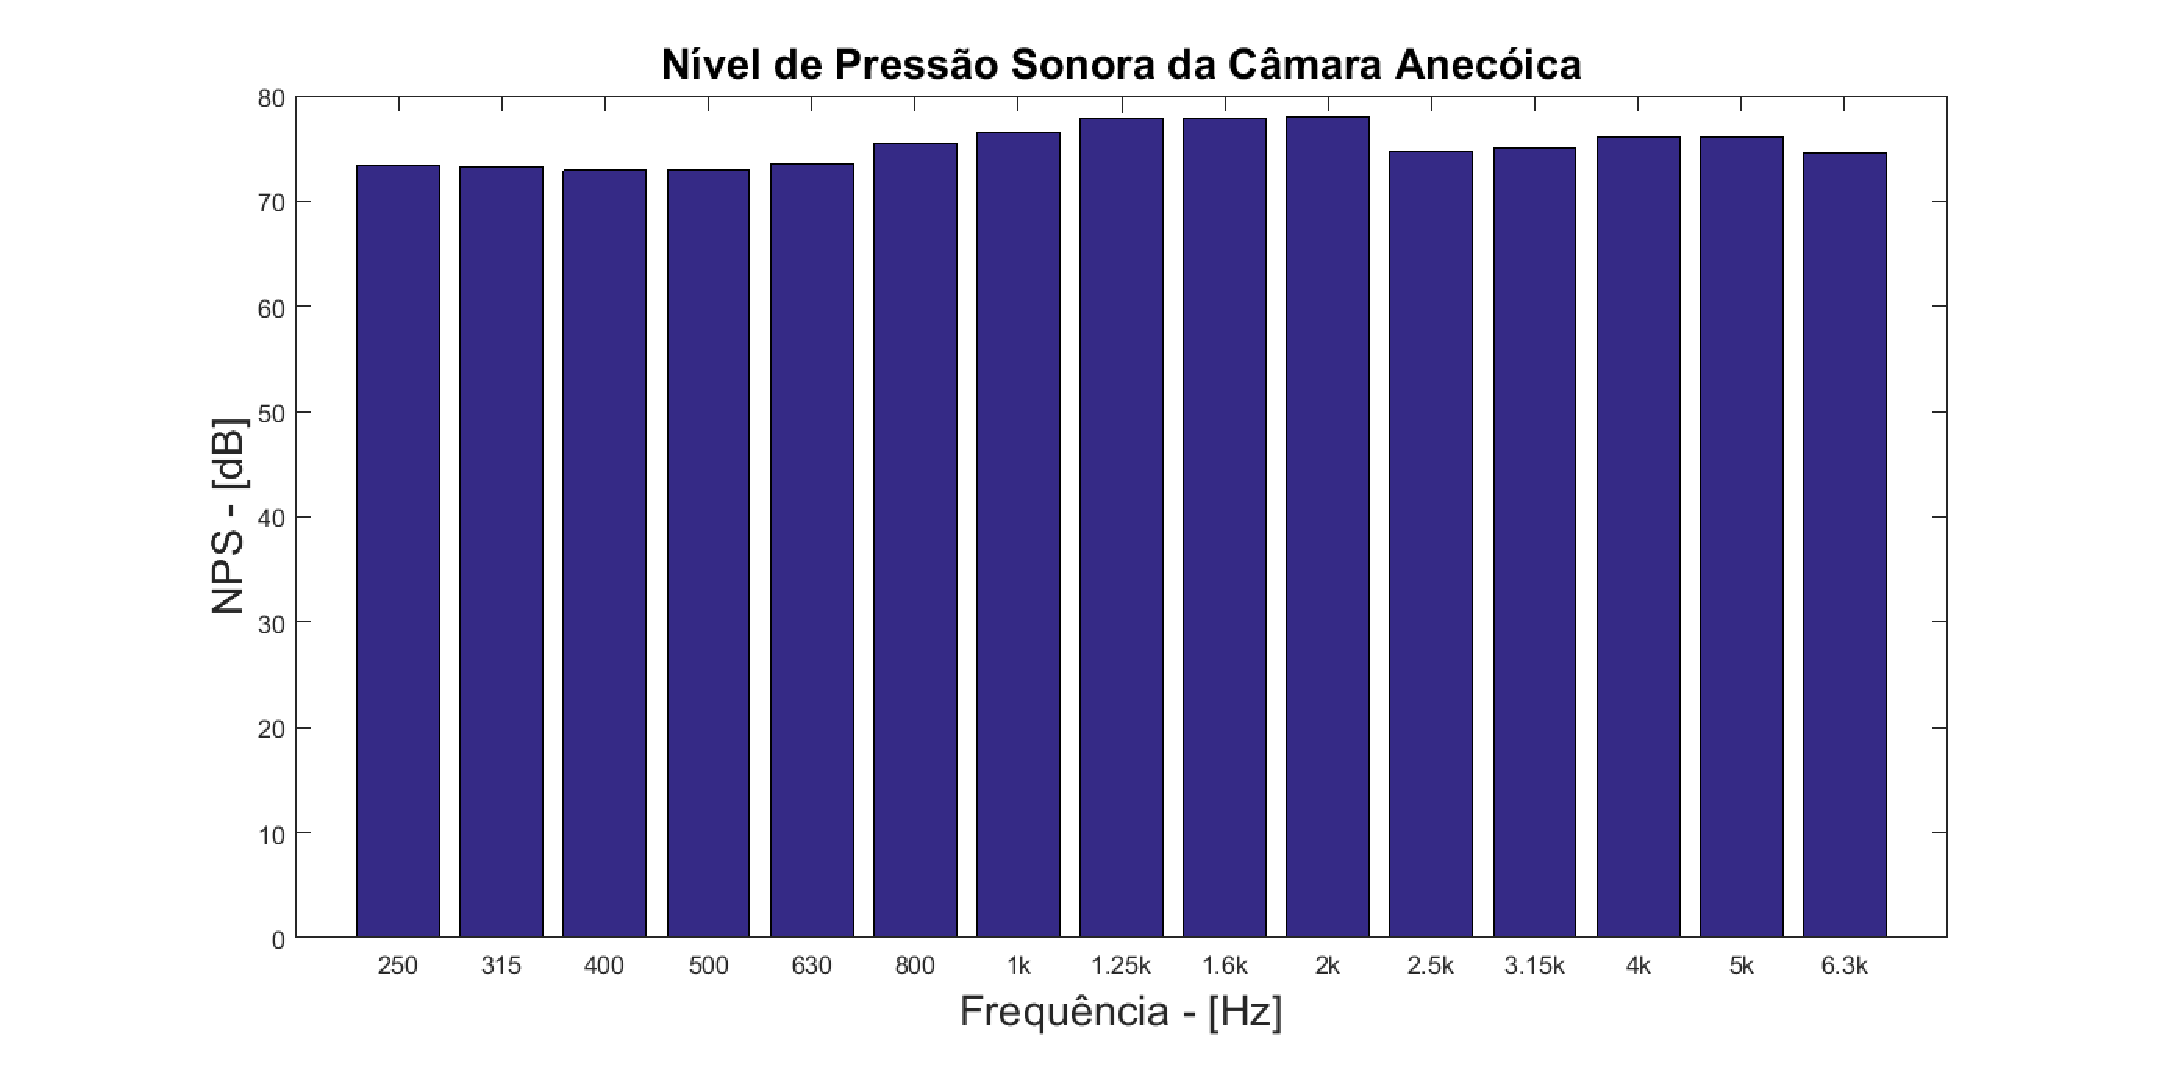
\includegraphics[width=1.6\textwidth]{figuras/P_anecoica.eps}
 %   \caption{Comparação das potências sonoras. Fonte: autoria própria.}
  %  \label{figura_8}
%\end{figure}


\chapter{Parte 2}\label{parte_2}

\section{B - Procedures} % (fold)
\label{sec:procedures}
	
	\subsection{1 - Define the number of necessary time steps NTS for an acoustic disturbance to propagate from the center
of the lattice until its boundaries. Remember that the lattice - as default in the provided Matlab code lbgk1.m - is 300 × 300 cells.} O tempo necessário para a perturbação chegar até a extremidade da $lattice$ é de $150 . \sqrt[2]{3}$. Esse cálculo é feito levando em consideração a distância $lattice$ de 150 e a velocidade de $lattice$ que é $\sqrt[2]{3}$.

\subsection{2 - Create an harmonic acoustic source in the center of the lattice. One way to accomplish that is to impose
an harmonic density fluctuation.}
\begin{lstlisting}
%% 6 - Begin the iteractive process
frequency_source = 1000; % Hz
amplitude_source = 0.001;
for ta = 1 : 150*sqrt(3)
    
    %% 6.1 - Propagation (streaming)
    lattice = stream_lattice(lattice);

    %% 6.2 - Get density
    lattice_distribution = lattice{1};
    density_total = sum(lattice_distribution,3);

    %% 6.2.1 - Source sound
    attice_distribution = lattice{1};
	size_lattice = size(lattice_distribution(:, :, 1));
	number_lines_lattice = size_lattice(1);
	number_columns_lattice = size_lattice(2);
    source_sound = lattice_distribution(number_lines_lattice/2, number_columns_lattice/2,9) + ...
    amplitude_source*sin(2*pi*frequency_source*(ta - 1)*lattice_time_step);
	lattice_distribution(number_lines_lattice/2, number_columns_lattice/2,9) = source_sound;
 	lattice = set_initial_disturbances(lattice, source_sound);   

    %% 6.3 - Collide
    lattice = collide_lattice(lattice, frequency_relaxation);
    
% Ploting the results in real time   
surf(density_total - 1), view(2), shading flat, axis equal, caxis([-.00001 .00001])
grid off
pause(.0001) 

end %  End main time Evolution Loop
\end{lstlisting}

\subsection{3 - Obtain the numerical result for the acoustic pressure field $p_{an}$ at ta = NTS along the lattice coordinate
vector x = [150 : 300, 150]. The numerical results should be obtained for three different wavelength
discretizations (d = 8, 16, and 25 cells per wavelength). One way to change the wavelength discretization
is to keep the lattice pitch ∆x constant and vary the source frequency $freq$. Calculate also the phase of
the source when ta = NTS at x = [150, 150]. Save the results for each discretization along with the
distance vector x.}

\begin{lstlisting}
%% 6 - Begin the iteractive process
wavelength_discretizations = [8 16 25];
frequency_source = physical_sound_velocity/ ... 
(dimension_x_voxel*wavelength_discretizations(1)); % Hz
amplitude_source = 0.001;
for ta = 1 : 150*sqrt(3)
    
    %% 6.1 - Propagation (streaming)
    lattice = stream_lattice(lattice);

    %% 6.2 - Get density
    lattice_distribution = lattice{1};
    density_total = sum(lattice_distribution,3);
    % Get pressure field in ta = NTS along
    lattice_pressure = 0;
    if ta == 259
    	lattice_pressure = lattice_sound_speed^2*density_total(150:300, 150);
    	figure;
		plot(lattice_pressure);
		xlabel('Distance in cells number','FontSize',20);
		ylabel('Lattice Pressure','FontSize',20);
		title('Waves with discretization 8 cells per wavelength','FontSize',20);
		%save lattice_pressure_d_25.mat lattice_pressure;
		phase_wave = 2*pi*frequency_source*(ta - 5)*lattice_time_step
    end

    %% 6.2.1 - Source sound
    attice_distribution = lattice{1};
	size_lattice = size(lattice_distribution(:, :, 1));
	number_lines_lattice = size_lattice(1);
	number_columns_lattice = size_lattice(2);
    source_sound = lattice_distribution(number_lines_lattice/2, number_columns_lattice/2,9) + ...
    amplitude_source*sin(2*pi*frequency_source*(ta - 1)*lattice_time_step);
	lattice_distribution(number_lines_lattice/2, number_columns_lattice/2,9) = source_sound;
 	lattice = set_initial_disturbances(lattice, source_sound);

    %% 6.3 - Collide
    lattice = collide_lattice(lattice, frequency_relaxation);
    
% Ploting the results in real time   
%surf(density_total - 1), view(2), shading flat, axis equal, caxis([-.00001 .00001])
%grid off
%pause(.00001)
ta
end %  End main time Evolution Loop
\end{lstlisting}

\begin{figure}[h!]
    \centering
 	\hspace{-2.5cm}
    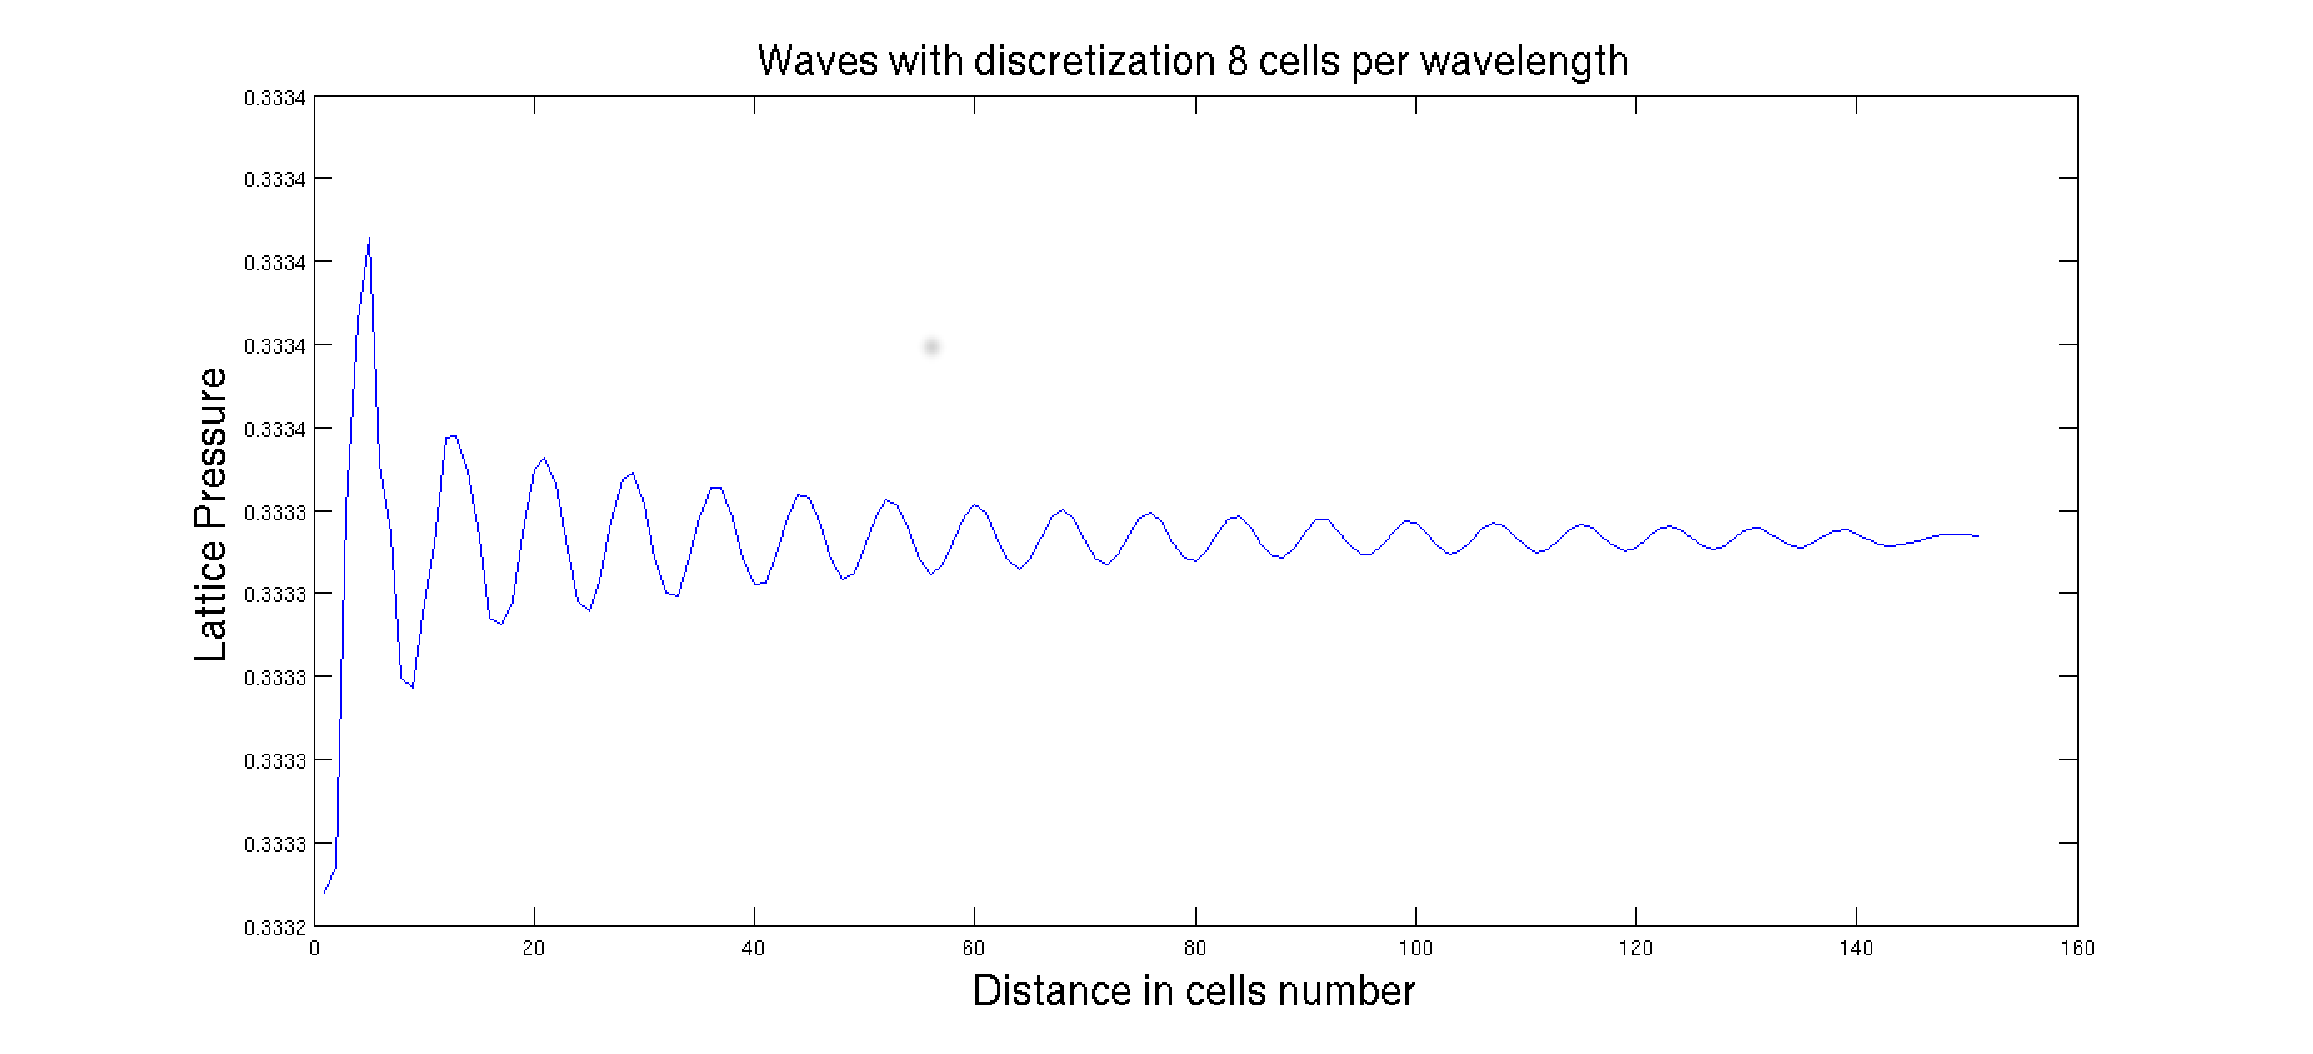
\includegraphics[width=1.2\textwidth]{figuras/pressure_graph_8_cells_discretization.eps}
    \caption{Discrezação com 8 células por comprimento de onda.}
\end{figure}

\begin{figure}[h!]
    \centering
   \hspace{-2.5cm}
    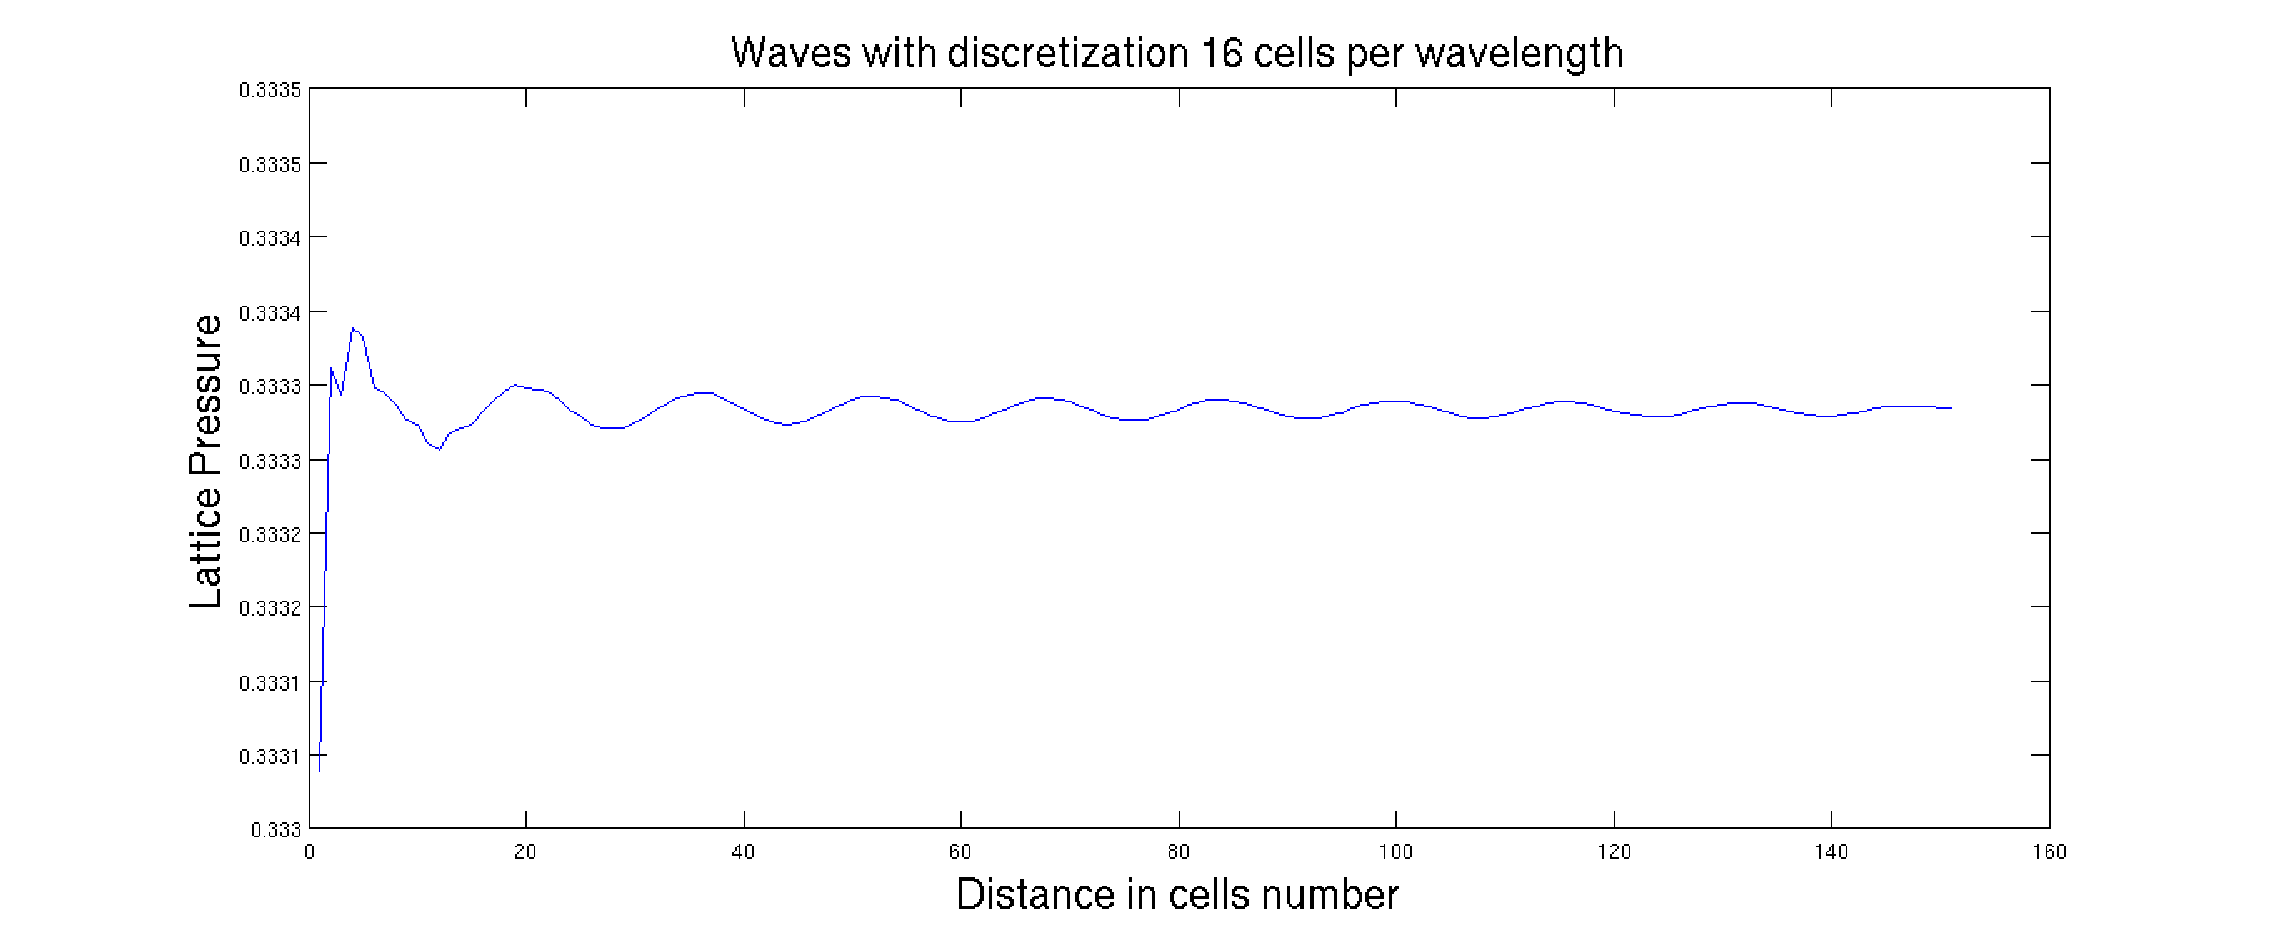
\includegraphics[width=1.2\textwidth]{figuras/pressure_graph_16_cells_discretization.eps}
    \caption{Discrezação com 16 células por comprimento de onda.}
\end{figure}

\begin{figure}[h!]
    \centering
    \hspace{-2.5cm}
    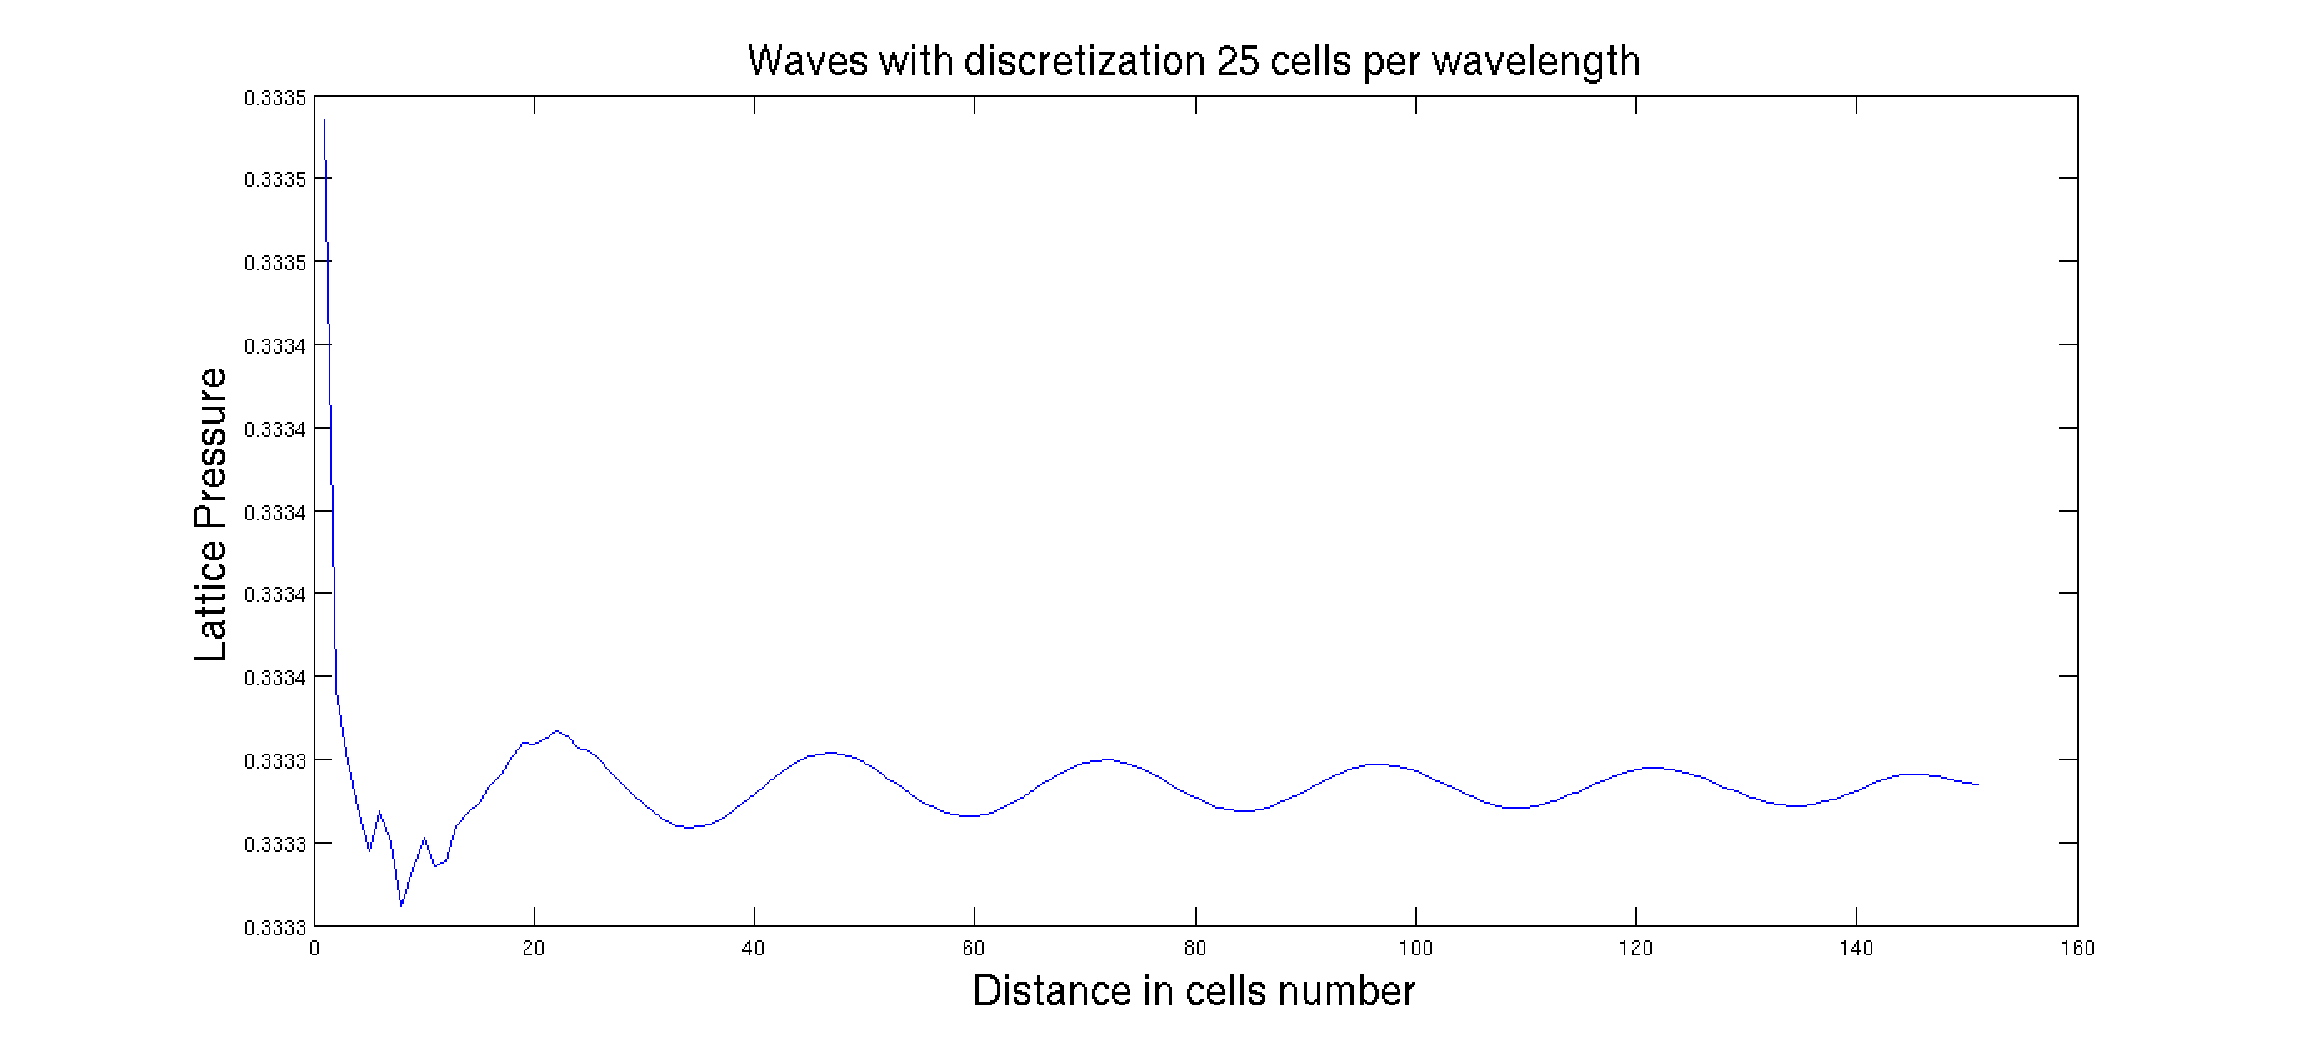
\includegraphics[width=1.2\textwidth]{figuras/pressure_graph_25_cells_discretization.eps}
    \caption{Discrezação com 25 células por comprimento de onda.}
\end{figure}

\subsection{4 - Calculate, in physical unities, the fluid kinematic viscosity, as well as the pressure amplitude at the
acoustic source corresponding to the default lattice variables used in the simulations. Use these values
to obtain the analytical pressure field p a as a function of the distance vector x based on Eq. (2). You
may use the Matalab function cylin wave.m for the calculations of p a . Save the resulting vectors of p a
for different source frequencies f req, and repeat this step using, at this time, the kinematic viscosity of
air in STP (vp = 1.5 × 10 −5 m 2 /s) to determine the analytical acoustic field p air as a function of the
distance vector x. Save it.}
\begin{lstlisting}
% 2D Lattice Boltzmann (BGK) model of a fluid.
%  c6  c2   c5  D2Q9 model. At each timestep, particle densities propagate
%    \  |  /    outwards in the directions indicated in the figure. An
%  c3 -c9 - c1  equivalent 'equilibrium' density is found, and the densities
%    /  |  \    relax towards that state, in a proportion governed by omega.
%  c7  c4   c8      Iain Haslam, March 2006.

clear all, clc
close all

%% 1 - Set lattice sizes
number_lines_lattice = 300; % cells in the y direction
number_columns_lattice = 300; % cells in the x direction

%% 2 - Set physical parameters (macro)
physical_sound_velocity = 340; % [m/s]
physical_density = 1.2; % [kg/m^3]
physical_dimension_max_x = .5; % [m]
physical_dimension_max_y = .5; % [m]
% voxel is a term to express a volume decribed in a pixel: volume + pixel = voxel
dimension_x_voxel = physical_dimension_max_x/number_columns_lattice; % defining dimension x in voxel
lattice_time_step = (1/sqrt(3))*dimension_x_voxel/physical_sound_velocity;

%% 3 - Set lattice parameters (meso - lattice unities)
frequency_relaxation = 1.9; % to 1.5e-5 physcosity 1.9998; 860e-5 = 1.9
time_relaxation = 1/frequency_relaxation;
lattice_average_density = 1;
lattice_sound_speed = 1/sqrt(3);
lattice_sound_speed_pow_2 = lattice_sound_speed^2;
lattice_viscosity = lattice_sound_speed_pow_2*(1/frequency_relaxation-0.5);
physical_viscosity = lattice_viscosity*(dimension_x_voxel^2)/lattice_time_step; % [m^2/s]

% 4 - Build lattice struct with D2Q9
lattice = build_lattice_D2Q9(number_lines_lattice, number_columns_lattice, lattice_average_density);

% 5 - Set initial disturbance
%initial_disturbance_density = 0.01;
%lattice = set_initial_disturbances(lattice, initial_disturbance_density);

%% 6 - Begin the iteractive process
wavelength_discretizations = [8 16 25];
frequency_source = physical_sound_velocity/ ... 
(dimension_x_voxel*wavelength_discretizations(3)); % Hz
amplitude_source = 0.001;
for ta = 1 : 150*sqrt(3)
    
    %% 6.1 - Propagation (streaming)
    lattice = stream_lattice(lattice);

    %% 6.2 - Get density
    lattice_distribution = lattice{1};
    density_total = sum(lattice_distribution,3);
    % Get pressure field in ta = NTS along
    lattice_pressure = 0;
    if ta == 259
    	lattice_pressure = lattice_sound_speed^2*(density_total(150:300, 150) - 1);
    	figure;
		plot(lattice_pressure);
		xlabel('Distance in cells number','FontSize',20);
		ylabel('Lattice Pressure','FontSize',20);
		title('Waves with discretization 25 cells per wavelength','FontSize',20);
		save lattice_pressure_d_25.mat lattice_pressure;
		phase_wave = 2*pi*frequency_source*(ta - 5)*lattice_time_step
		%physical_viscosity = 1.5e-5;
		%0.001 => pascal
		%[p pos]=cylin_wave();
		%(1/sqrt(3))/20,physical_viscosity,1/sqrt(3),0.001/20,1:150,pi/2
		%[analytical_pressure x] = cylin_wave(frequency_source, physical_viscosity, ...
		%physical_sound_velocity, amplitude_source, 1:number_columns_lattice/2, phase_wave);
		frequency_source_analytical = lattice_sound_speed/ ... 
		(wavelength_discretizations(3));
		[analytical_pressure x] = cylin_wave(frequency_source_analytical, ... 
		physical_viscosity, lattice_sound_speed, ...
		amplitude_source/wavelength_discretizations(3), 1:number_columns_lattice/2, 0);

		figure;
		plot(lattice_pressure);
		hold on;
		plot(analytical_pressure, 'r');
		%xlabel('Distance in cells number','FontSize',20);
		%ylabel('Lattice Pressure','FontSize',20);
		%title('Waves with discretization 25 cells per wavelength','FontSize',20);
    end

    %% 6.2.1 - Source sound
    attice_distribution = lattice{1};
	size_lattice = size(lattice_distribution(:, :, 1));
	number_lines_lattice = size_lattice(1);
	number_columns_lattice = size_lattice(2);
    source_sound = lattice_distribution(number_lines_lattice/2, number_columns_lattice/2,9) + ...
    amplitude_source*sin(2*pi*frequency_source*(ta - 1)*lattice_time_step);
	lattice_distribution(number_lines_lattice/2, number_columns_lattice/2,9) = source_sound;
 	lattice = set_initial_disturbances(lattice, source_sound);

    %% 6.3 - Collide
    lattice = collide_lattice(lattice, frequency_relaxation);
    
% Ploting the results in real time   
%surf(density_total - 1), view(2), shading flat, axis equal, caxis([-.00001 .00001])
%grid off
%pause(.00001)
ta
end %  End main time Evolution Loop
\end{lstlisting}

\subsection{5 - In a single figure, plot pan(x) for each discretization scheme, as well as their respective analytical solution pa(x).} 

\begin{figure}[h!]
    \centering
    \hspace{-2.5cm}
    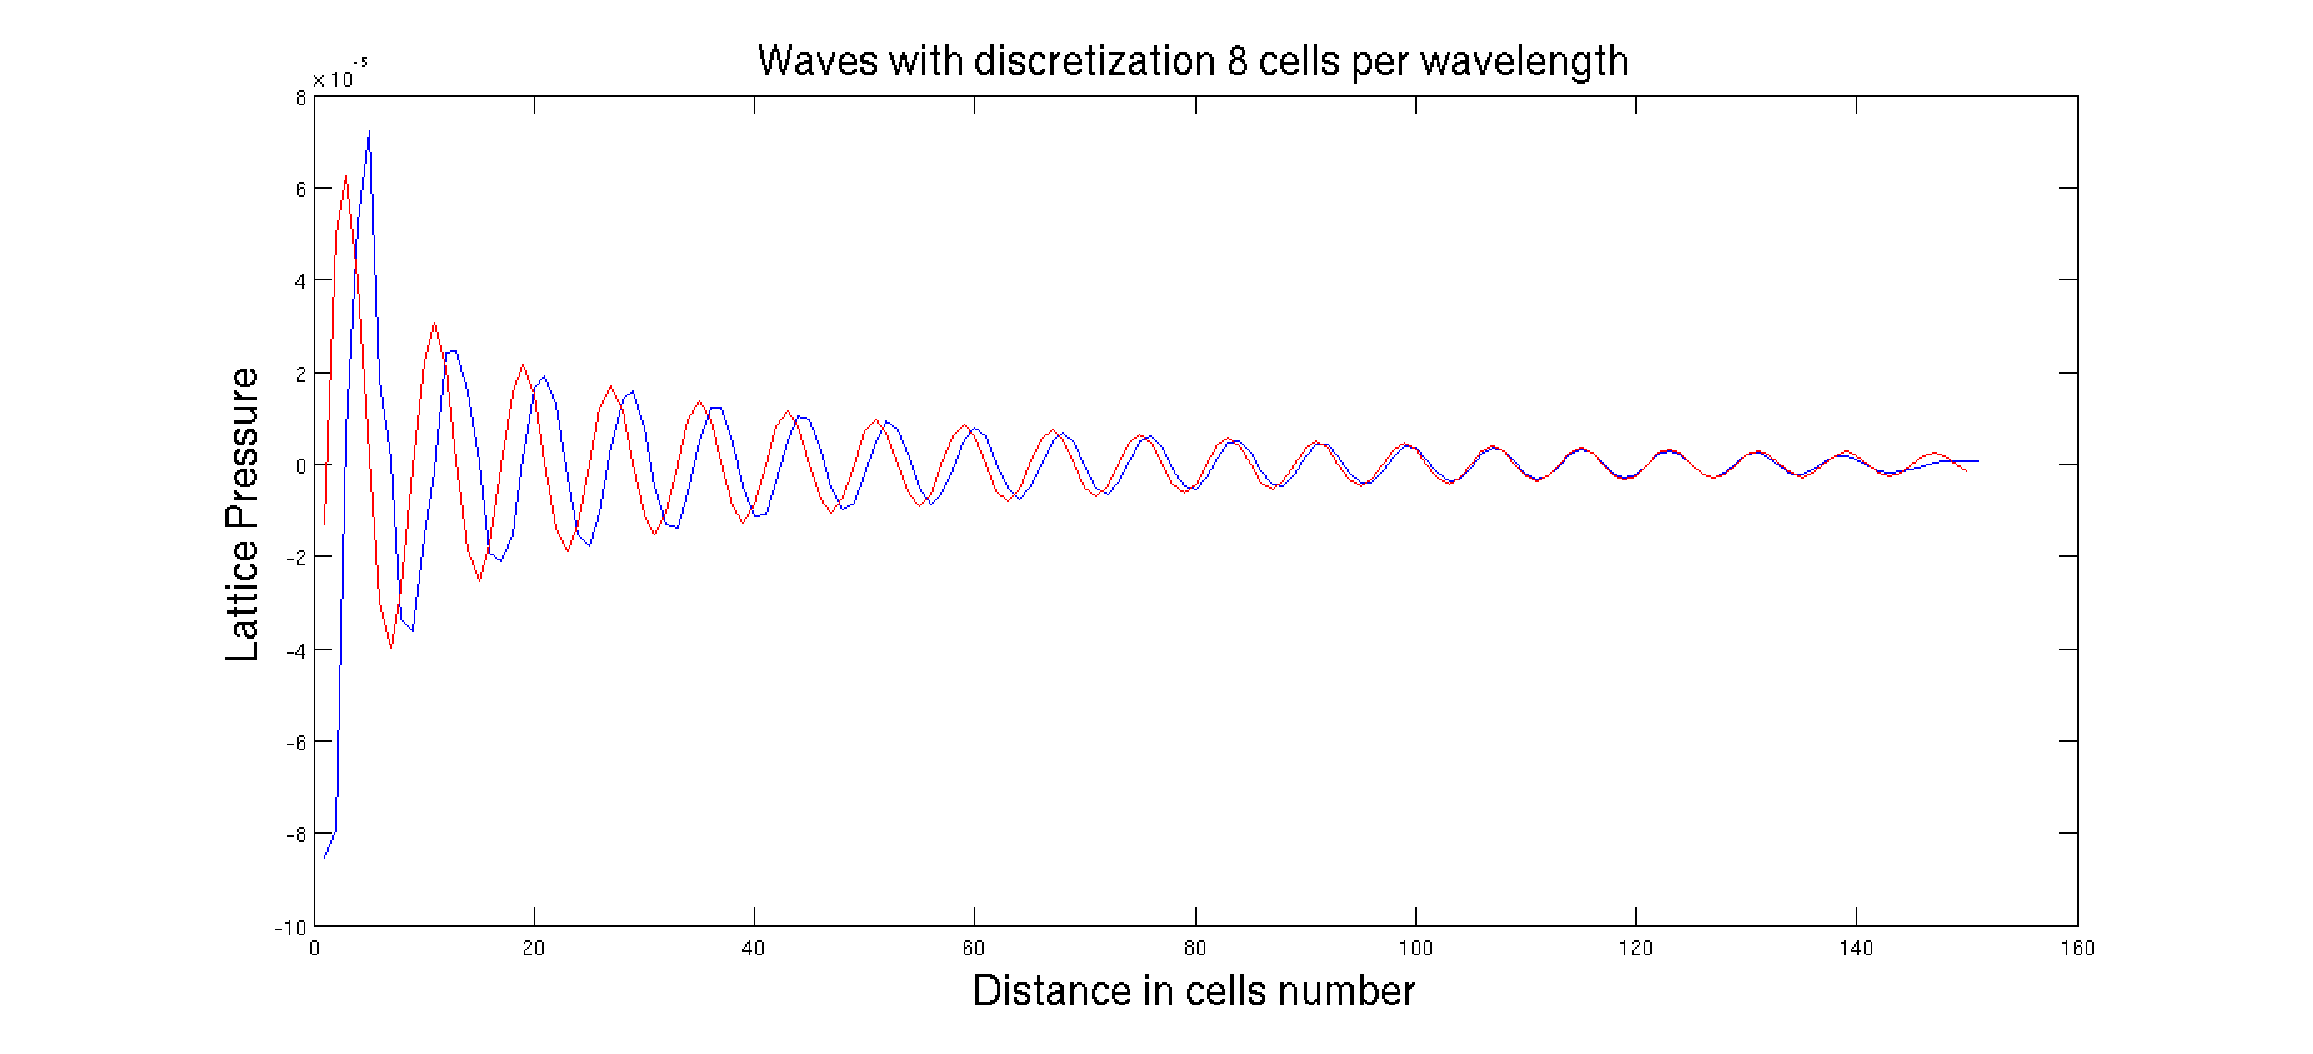
\includegraphics[width=1.2\textwidth]{figuras/compare_8_cells_discretization.eps}
    \caption{Comparação da solução analítica com 8 células por comprimento de onda.}
\end{figure}

\begin{figure}[h!]
    \centering
    \hspace{-2.5cm}
    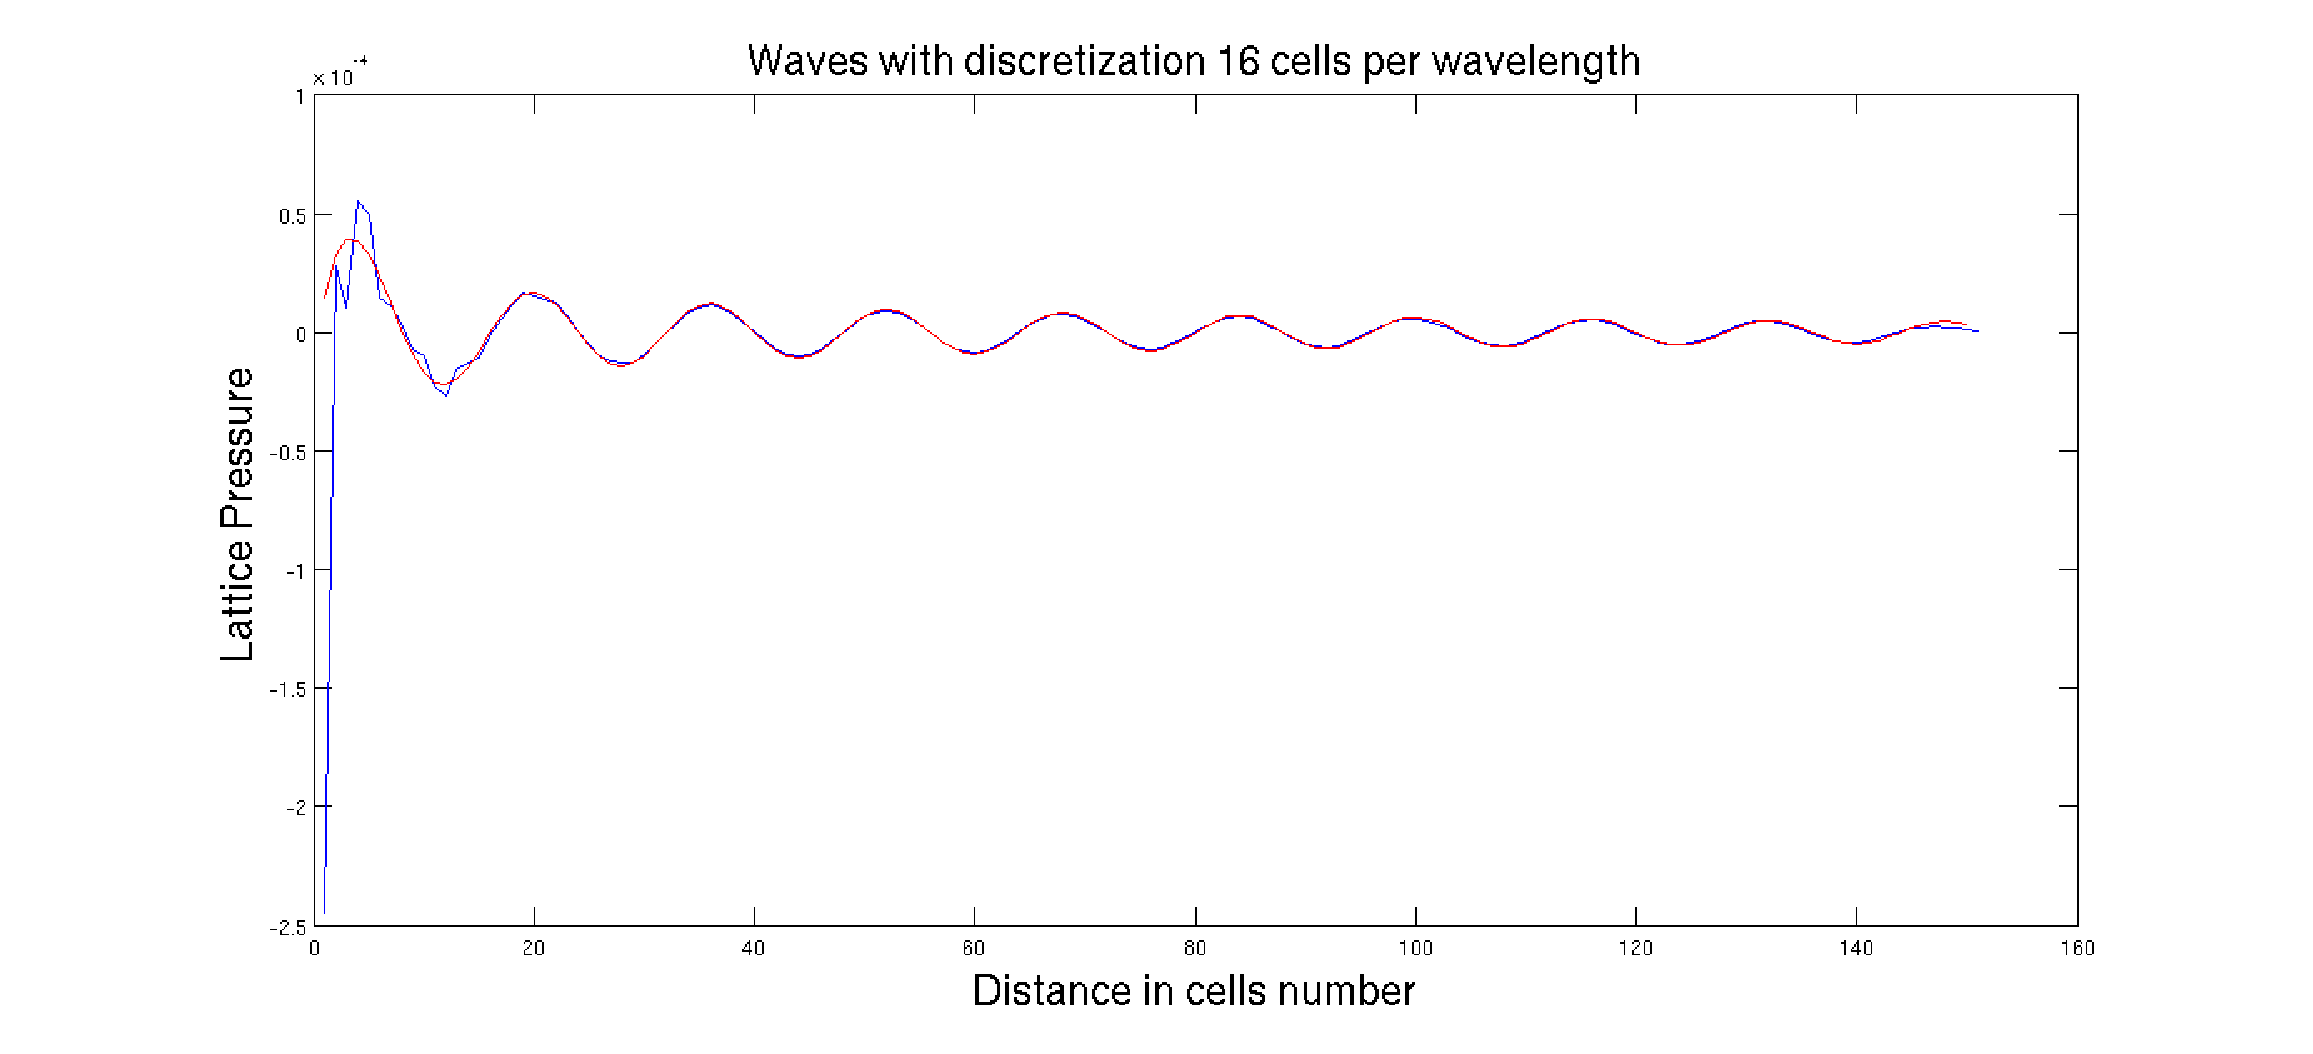
\includegraphics[width=1.2\textwidth]{figuras/compare_16_cells_discretization.eps}
    \caption{Comparação da solução analítica com 16 células por comprimento de onda.}
\end{figure}

\begin{figure}[h!]
    \centering
    \hspace{-2.5cm}
    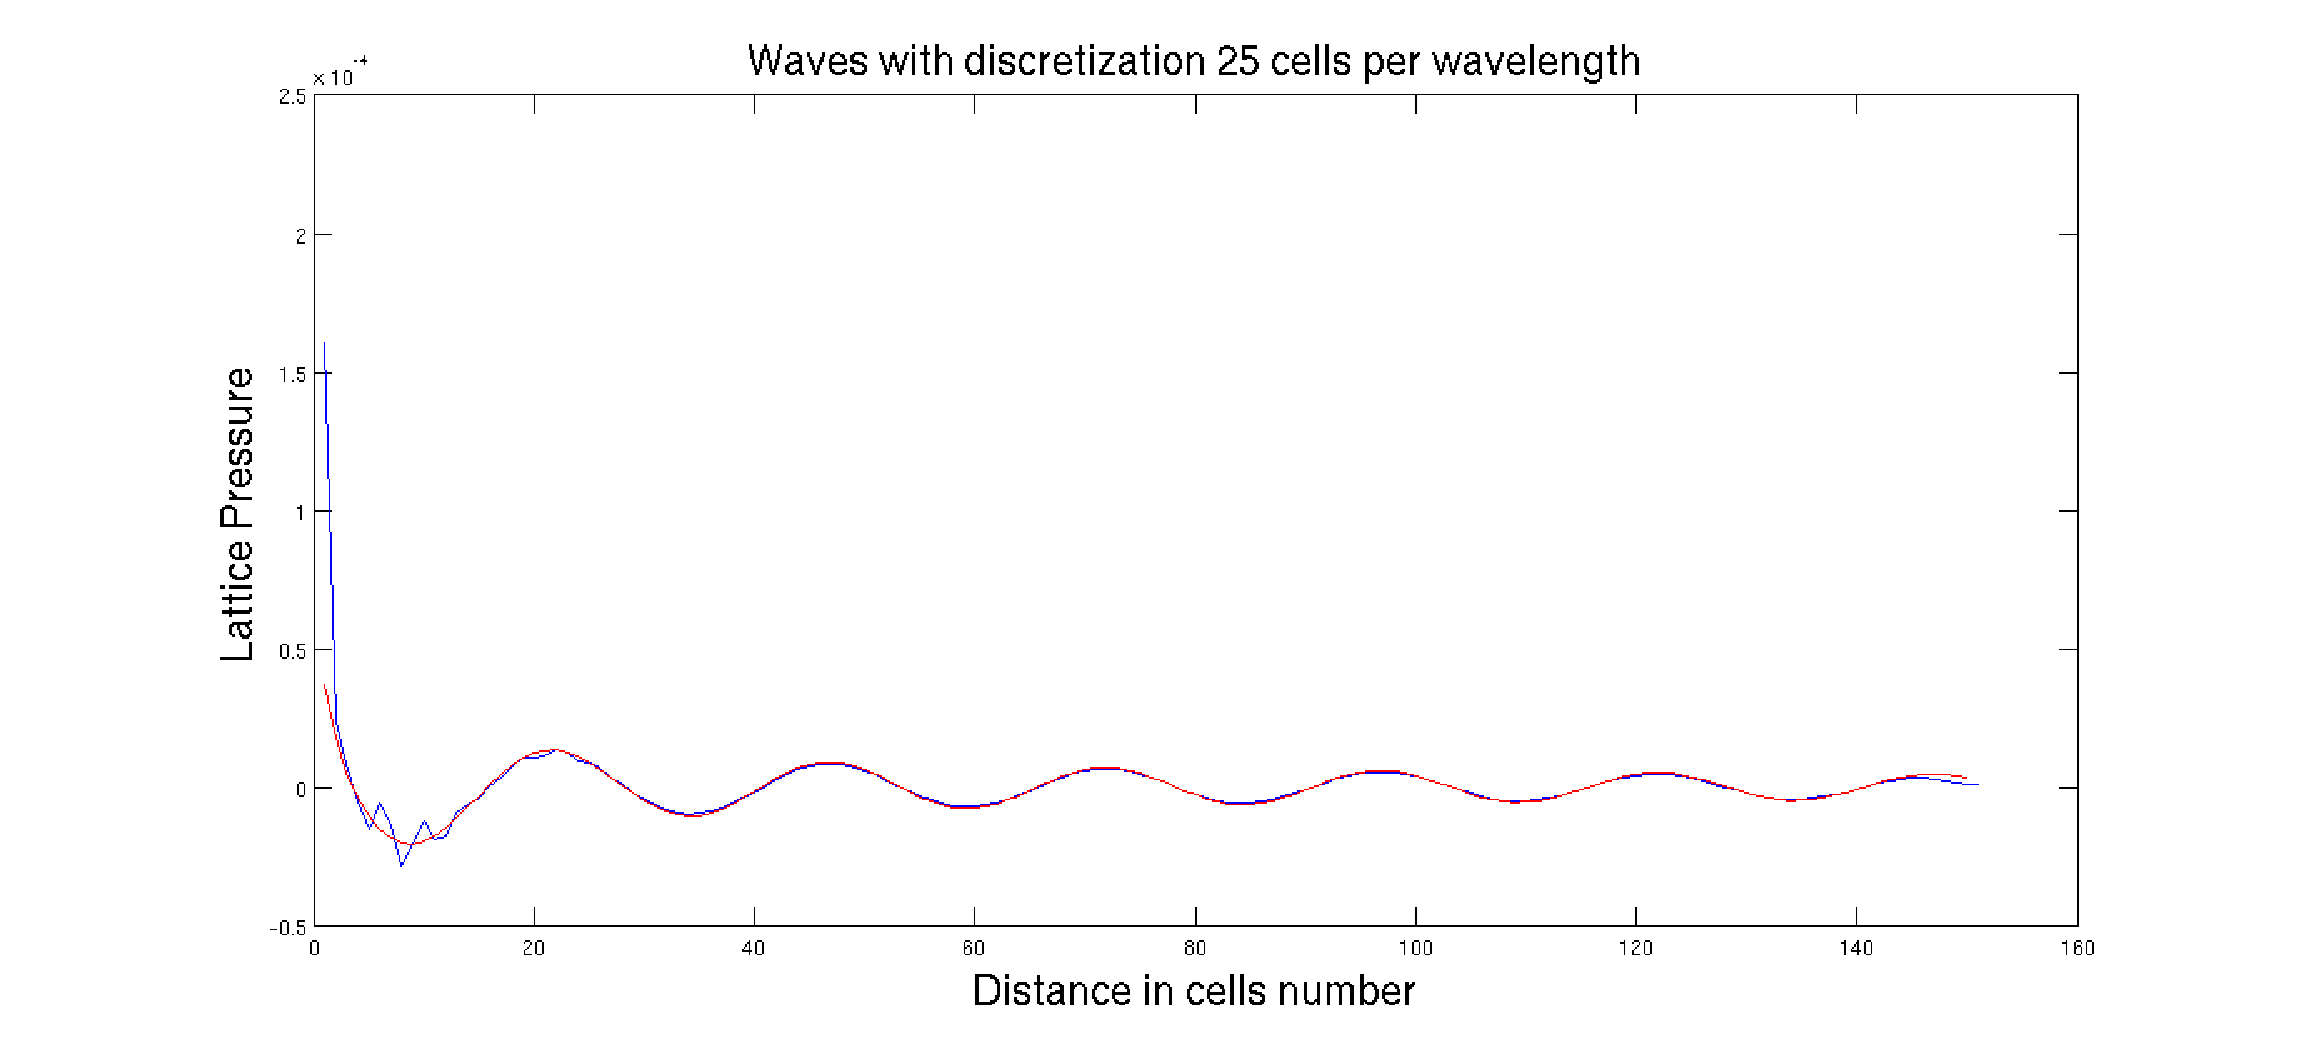
\includegraphics[width=1.2\textwidth]{figuras/compare_25_cells_discretization.eps}
    \caption{Comparação da solução analítica com 25 células por comprimento de onda.}
\end{figure}

\subsection{6 - In one figure, compare the different results obtained for p a (x) and p air (x).}
\begin{figure}[h!]
    \centering
    \hspace{-2.5cm}
    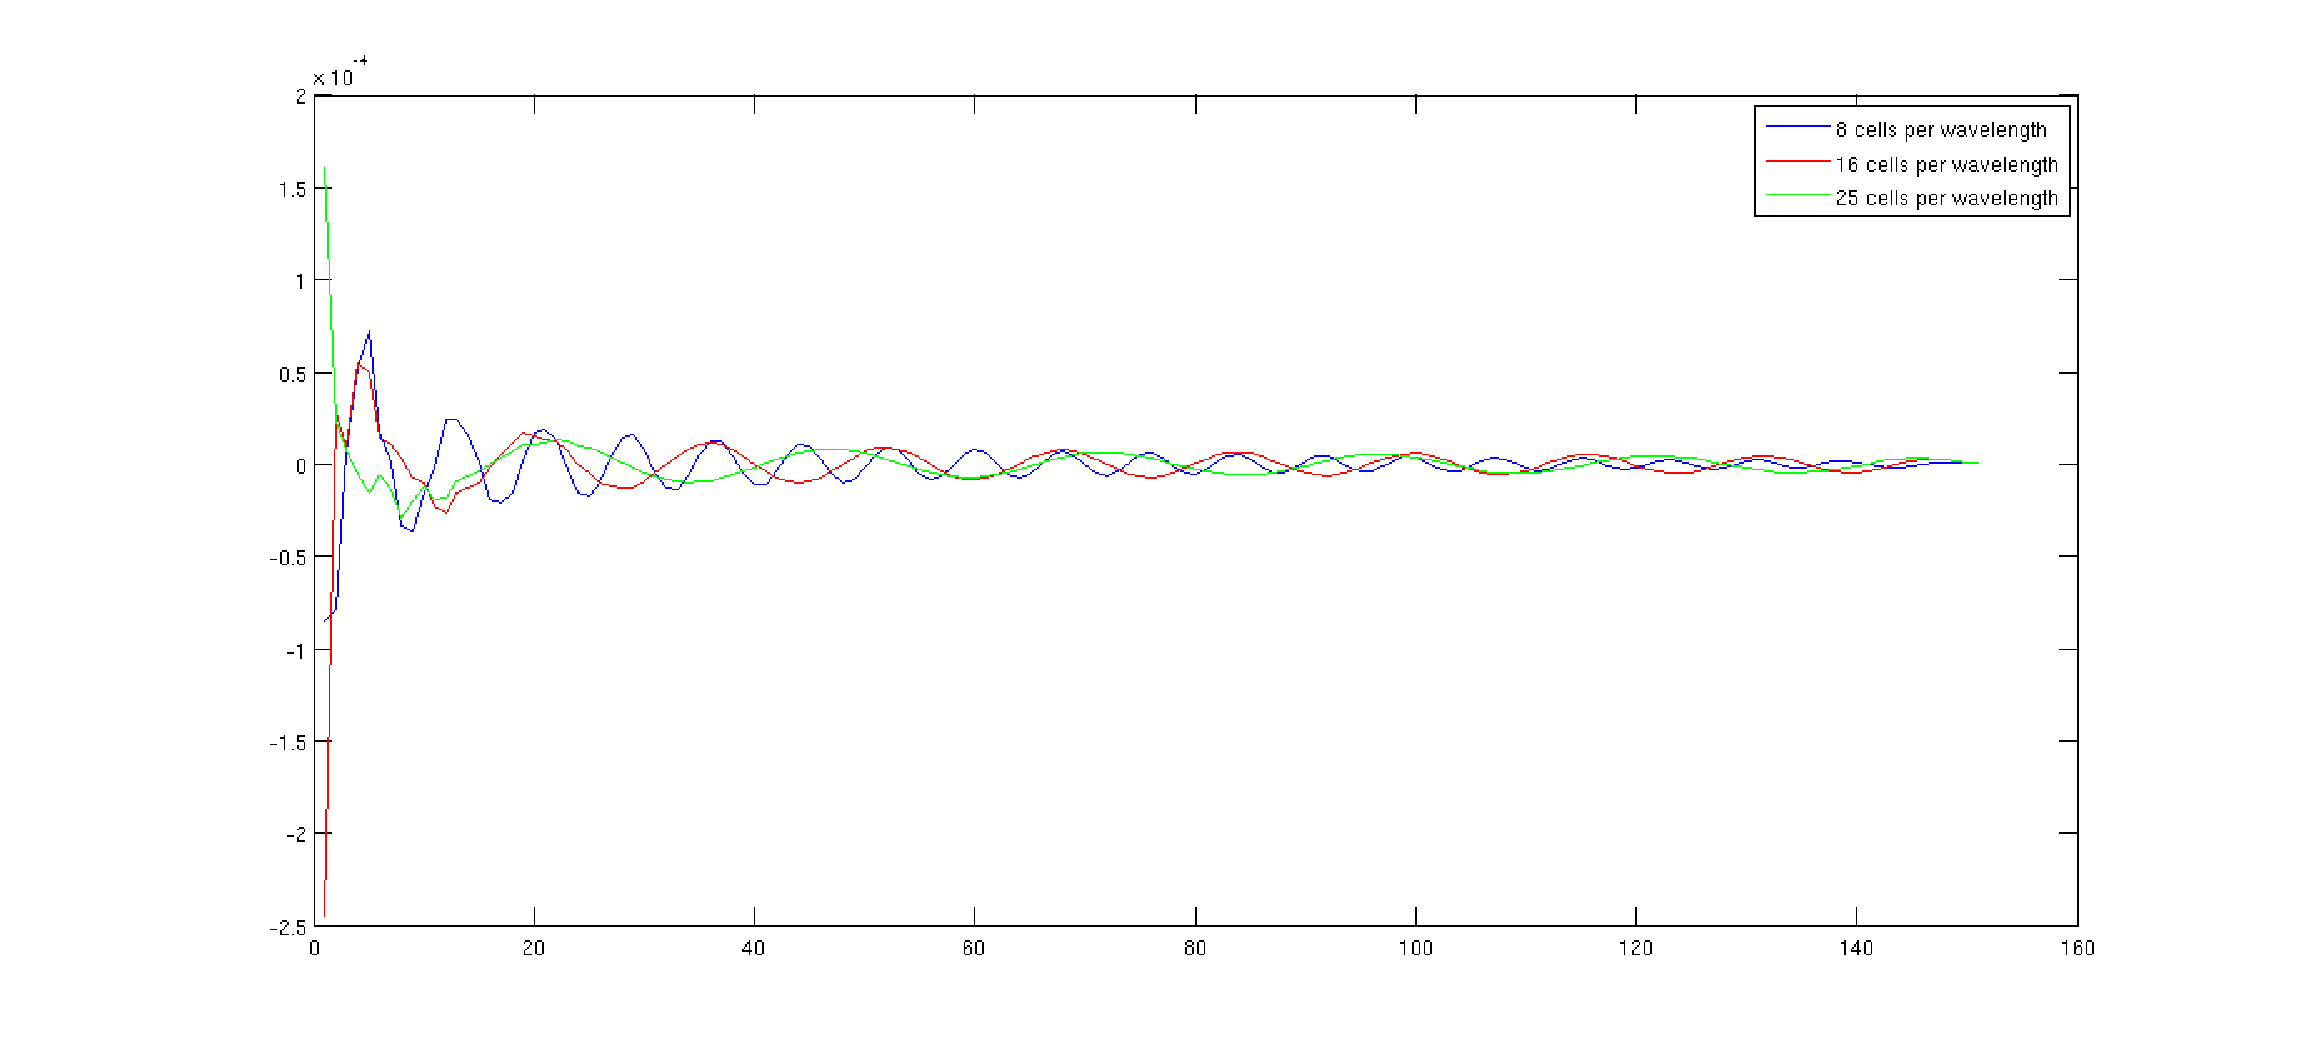
\includegraphics[width=1.2\textwidth]{figuras/all_in_one.eps}
    \caption{Comparação das simulações de vários comprimentos de onda.}
\end{figure}

\section{C - Questions} % (fold)

\subsection{1 - What is the observed effect of a low discretization scheme? Do these results qualitatively agree with
the analysis conducted by Wilde (2006) with respect to wave dissipation (see slides from the last class)?
Please, justify.} 
Para uma baixa discretização houve uma suavização da curva em relação a solução analítica porém a curva da simulação se encontra retraída em alguns pontos. Esse fez com que somente alguns pontos se encaixaram na curva de solução analítica.

\subsection{2 - For high discretization schemes (16, 25 cells per wavelength) a slight disagreement between pan(x) and
pa(x) should be noticeable when the wave approaches the lattice boundary. Can you explain why?}
Há uma descontinuidade pois não há uma condição de contorno definida no problema, ou seja, as células de densidades que vão para a fronteira são eliminadas do lattice. Esse fato pode ser observado na função de deslocamento (propagação) de células.
 
\subsection{3 - Due to the limitations of the LBGK model, the physical viscosity used in the simulations is O(2) higher
than the kinematic viscosity of air in normal conditions. Even so, the error between pan(x), pa(x),
pair (x) reasonably small. Can you draw any conclusions over this fact?} Pode-se concluir que pequenas variações a frequência de relaxação de lattice causam grandes variações na viscosidade física, um bom exemplo disso é:
\begin{itemize}
	\item 860e-5 de viscosidade física equivale 1.9 de taxa de relaxação;
	\item 1.5e-5 de viscosidade física equivale 1.9998 de taxa de relaxação.
\end{itemize}
 Obs: quando se chega taxa de relaxação de 2.0 ou maior a malha $lattice$ possui comportamentos inesperáveis.


 \section{D - OpenLB}
 \begin{lstlisting}
 #include "olb2D.h"
#ifndef OLB_PRECOMPILED // Unless precompiled version is used
    #include "olb2D.hh" // include full template code
#endif

using namespace olb;

// Some C++ libraries wich are for the example and others
#include <vector>
#include <cmath>
#include <iostream>
#include <iomanip> 
#include <fstream>
#include <string>
#include <Magick++.h> 
#include <unistd.h>
#include <thread>  
#include <math.h>
#define PI 3.14159265

using namespace olb;
using namespace olb::descriptors; // accessed in the examples
using namespace olb::graphics; 
using namespace std; // Namespace of standard C++ library

// Definindo a minha lattice
// Aqui eu posso definir tambem outros escalares naturais como
// forcas. Para tais coisas memoria deve ser alocada na malha de lattice.
#define LATTICE D2Q9Descriptor
typedef double T;
int nx = 300;
int ny = 300;
int numIter = 250; // numero de iteracoes ou passos
T omega = 1.98; // viscosidade
T r = 30.; // raio do circulo
T cs = 1/sqrt(3); // lattice speed of sound
T cs2 = cs*cs; // Squared speed of sound cl^2 

int main(int argc, char* argv[]){

    std::string ss;
    olbInit(&argc, &argv);
    //Ele pede para inserir a principal parte do codigo aqui, mas oq?
    BlockLattice2D<T, LATTICE> lattice(nx, ny); // Aqui o bloco de malha de lattice  nxXnyX9 eh instanciado
    //Tipo de dinanimca, pode-se colocar perda de massa por exemplo
    BGKdynamics<T, LATTICE> bulkDynamics(omega, instances::getBulkMomenta<T, LATTICE>());
    //Deve-se indicar em quais lugares da malha lattice vai ocorrer a dinamica: nesse caso com todos os pontos
    lattice.defineDynamics(0,nx-1,0,ny-1,&bulkDynamics);
    
    //Setar a condicao inicial de equilibrio, espalhando as densidades na malha
    //Nesse caso tera uma distribuicao mais densa num circulo de raio r
    T rho = 1., u[2] = {0.,0.};
    for(int iX = 0; iX<nx; ++iX){
        for(int iY = 0; iY<ny; ++iY){
            lattice.get(iX, iY).iniEquilibrium(rho, u);
        }
    }

    // As colisoes definidas em bulkDynamics sao efetivadas aqui em cada celula
    T rho_varia;
    T lattice_speed_sound = 1/sqrt(3);
    T A_amplitude = 0.001;
    for(int iT = 0; iT <= numIter; ++iT){

        //Fluxo, true indica que as bordas sao periodicas
        //lattice.collideAndStream(true);
        lattice.stream();

        FILE * pFile;
        pFile = fopen ("space_points_1.txt","w");
        cout << "escrevendo resultado final" << endl;
        for (int i = 149; i <= 299; i++){
            double sum = (lattice.get(i, 149).computeRho()-1)*cs2;
            fprintf (pFile, "%.10f ", sum);
        }
        fclose (pFile);

        rho_varia = 1. + A_amplitude*sin(2*PI*(lattice_speed_sound/20)*iT);
        //printf("%f\n", rho_varia);
        lattice.get(149, 149).defineRho(rho_varia);

        lattice.collide();

    }
}
 \end{lstlisting}

\begin{figure}[h!]
    \centering
    \hspace{-2.5cm}
    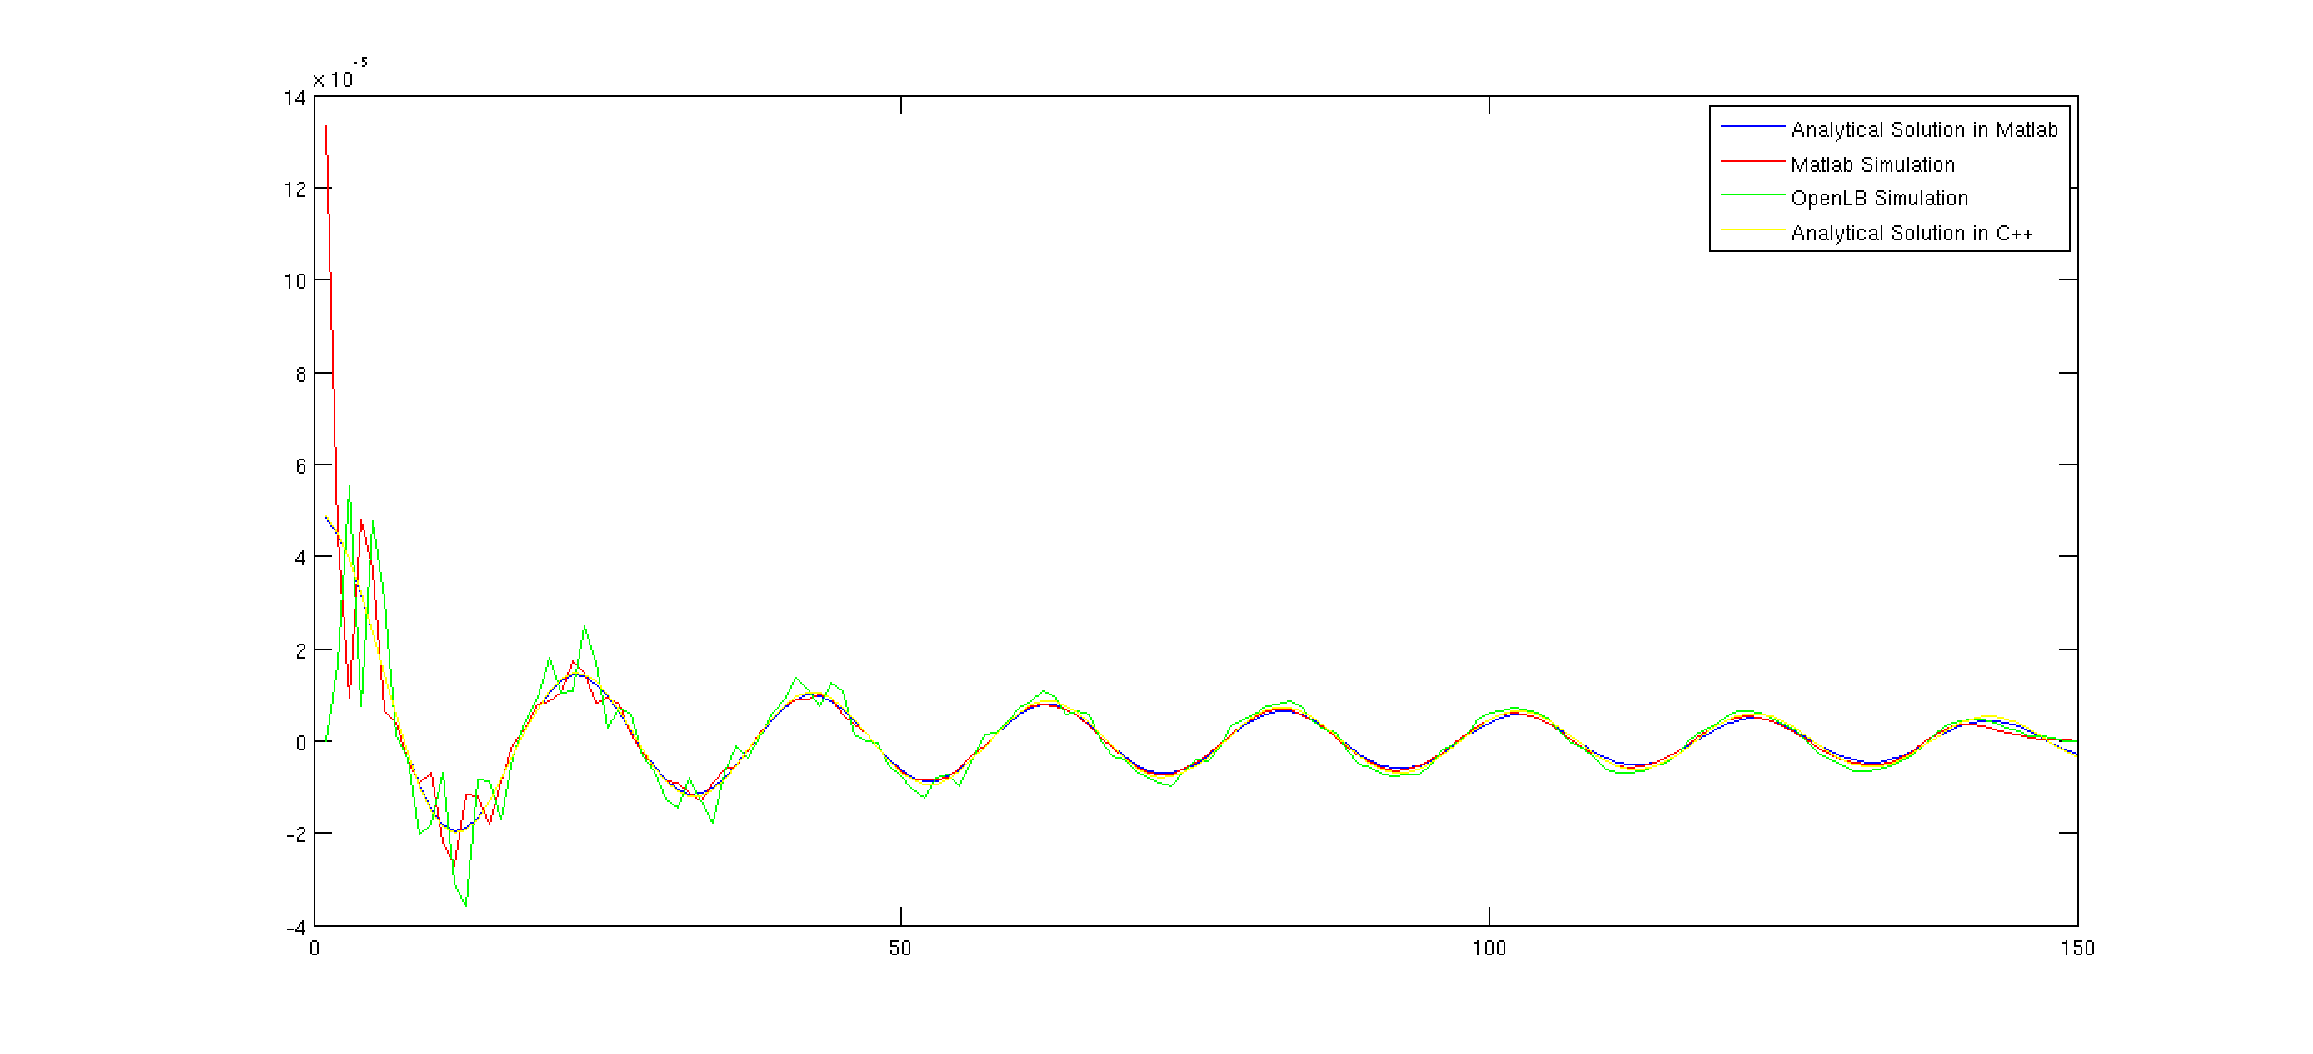
\includegraphics[width=1.2\textwidth]{figuras/openlb.eps}
    \caption{Comparação entre solução analítica escrita em MATLAB e C++ com as simulações no MATLAB e OpenLB.}
\end{figure}




